% Consolidated tables matching the manuscript numbering (Tables 1--2, 5).
% Tables 3--4 appear in \texttt{results.tex} with the subsections that discuss them.

\begin{table}[p]
  \centering
  \caption{Validation results across domains.}
  \label{tab:validation}
  \small
  \begin{tabular}{@{}llccccl@{}}
    \toprule
    \textbf{Domain} & \textbf{Tier} & \textbf{$n$ studies} & \textbf{Mean $\eta$} & \textbf{SD} & \textbf{\% with $\eta>1$} & \textbf{Data source} \\
    \midrule
    Sports (Rugby)      & Primary    & \PEFrugbyNkpis  & \PEFrugbyMeanEta  & \PEFrugbySdEta  & \PEFrugbySuccess\%  & {URC} \\
    Sports (Football)   & Primary    & \PEFfootNkpis   & \PEFfootMeanEta   & \PEFfootSdEta   & \PEFfootSuccess\%   & English Championship \\
    Healthcare          & Supporting & $\PEFhealthN^{\dagger}$ & \PEFhealthMeanEta & 0.04$^{\dagger}$ & \PEFhealthSuccess\% & \cite{nhanes2017pbxo} \\
    Clinical Genomics   & Supporting & $\PEFgenomicsN^{\ddagger}$ & \PEFgenomicsMeanEta & \PEFgenomicsSdEta & \PEFgenomicsSuccess\% & \cite{brunner2014earlybreast,geoGSE47462} \\
    Finance             & Supporting & \PEFfinanceN    & \PEFfinanceMeanEta & \PEFfinanceSdEta & \PEFfinanceSuccess\% & Yahoo Finance \\
    Manufacturing       & Supporting & $\PEFmfgN^{\S}$ & \PEFmfgMeanEta    & \PEFmfgSdEta    & \PEFmfgSuccess\%    & \cite{openml752bosch} \\
    \bottomrule
  \end{tabular}
  \normalsize

  \medskip
  \begin{minipage}{0.95\linewidth}\small
    \textit{Note:} Landscape efficiency rate: proportion of units with $\hat\eta>1$ (\cref{sec:outcome_defs}). The $n$ studies column is the number of PEF units, not a participant count: healthcare is one paired study of $N=10{,}352$ participants. $^{\dagger}$Paired {NHANES} oscillometric records (systolic vs diastolic, first reading); SD column gives a bootstrap standard error for the pooled $\eta$ (not a cross-unit sample SD). $^{\ddagger}$Genes in the ranked subset of the {GSE47462} paired design (see Methods). $^{\S}$Axis-wise paired process features per {Bosch} production cycle ({OpenML} 752); SD is the sample {SD} of $\eta$ across pairings. Primary empirical tier: landscape characterisation in Figures~\ref{fig:pef_landscape}--\ref{fig:info_surface} and Supplementary~\cref{fig:si_kpi_labelled,fig:si_ipred_vs_dml}; mechanistic confirmation via \cref{fig:pef_ml,tab:exemplars}. Supporting tier: parameter estimation and PEF calculation summarised here and in \cref{sec:results}; mean $(\kappa,\rho)$ overlay in \cref{fig:pef_landscape}.
  \end{minipage}
\end{table}

\begin{table}[p]
  \centering
  \caption{Quadrant taxonomy and practical guidance.}
  \label{tab:quadrants}
  \begin{tabular}{@{}lllll@{}}
    \toprule
    \textbf{Q} & \textbf{Parameters} & $\eta$ & $I(X;Y)$ & \textbf{Recommendation} \\
    \midrule
    Q1 & $\kappa>1$, $\rho>0$  & $>1$  & High     & Use relative features \\
    Q2 & $\kappa<1$, $\rho>0$  & $>1$  & Moderate & Use relative features \\
    Q3 & $\kappa<1$, $\rho<0$  & $<1$  & Low      & Prefer absolute features \\
    Q4 & $\kappa>1$, $\rho<0$  & $<1$  & Variable & Analyse both $\eta$ and $I(X;Y)$ \\
    \bottomrule
  \end{tabular}

  \medskip
  \begin{minipage}{0.95\linewidth}\small
    \textbf{Examples:} Q1, market-adjusted returns, paired clinical trials; Q2, control charts, quality metrics; Q3, high-volume anti-correlated sports KPIs; Q4, asymmetric head-to-head comparisons (some sports KPIs; competitive business).
  \end{minipage}
\end{table}

\begin{table}[p]
  \centering
  \caption{Boundary behaviour (illustrative).}
  \label{tab:boundary}
  \begin{tabular}{@{}lccc@{}}
    \toprule
    \textbf{Condition} & $\eta$ & $I(X;Y)$ & \textbf{Interpretation} \\
    \midrule
    $\kappa=1$, $\rho=0$ (Fisher) & 1.000 & 0.056 & Baseline: independent, equal variances \\
    $\kappa\to 0$                 & 1.000 & 0.108 & Entity B negligible \\
    $\kappa\to\infty$             & 1.000 & $\to 0$ & Signal drowned in noise \\
    $\rho\to -1$ ($\kappa=1$)     & 0.500 & 0.028 & Maximum variance amplification \\
    $\rho\to +1$ ($\kappa=1$)     & $\to\infty$ & $\to 1$ & Perfect cancellation of noise \\
    \bottomrule
  \end{tabular}

  \medskip
  \begin{minipage}{0.95\linewidth}\small
    \textit{Note:} $I(X;Y)$ computed with $\delta/\sigma_{\mathrm{A}}=1$.
  \end{minipage}
\end{table}

\begin{figure}[p]
  \centering
  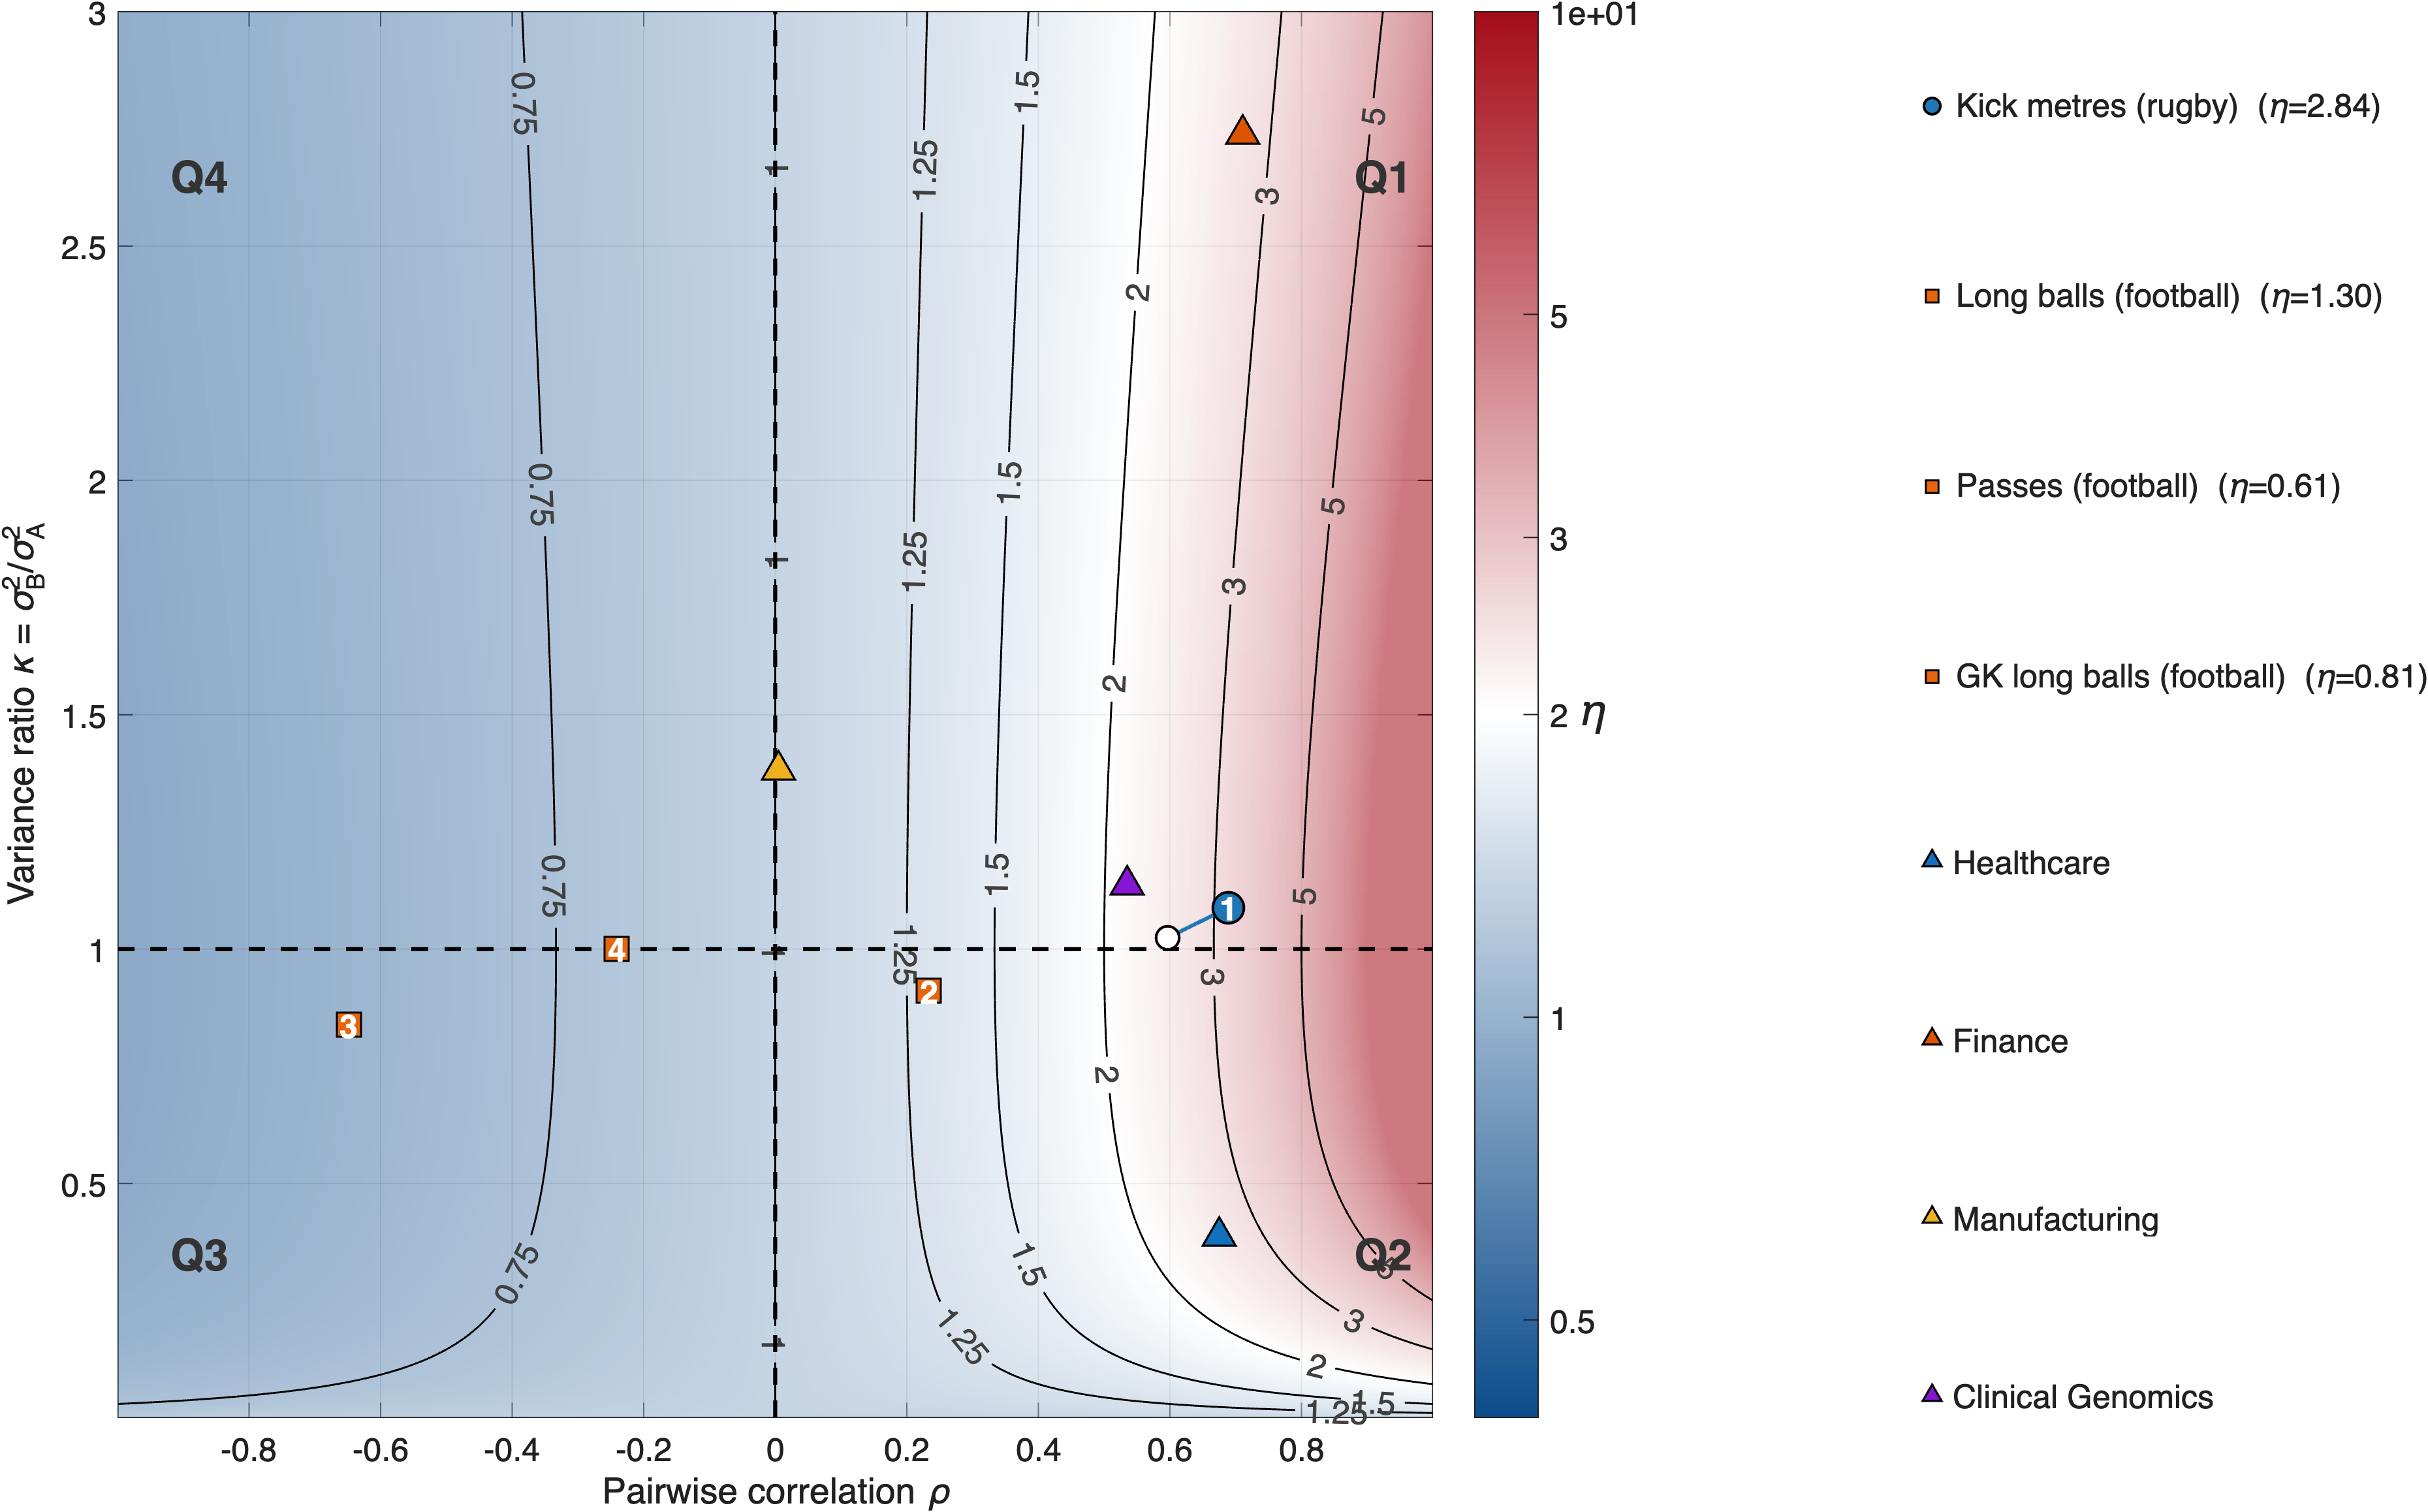
\includegraphics[width=0.95\linewidth]{figures/Figure_1.png}
  \caption{PEF landscape: $\eta$ as a function of $\rho$ and $\kappa$, with four quadrants labelled.
    Background shading uses a $\log_{10}$ colour mapping of $\eta$ (tick labels show $\eta$) so that
    the admissibility blow-up as $\rho\to +1$ (Supplementary~\cref{sec:si_maths}) remains visible; contour
    lines are in raw $\eta$.
    The dotted curve marks the admissibility boundary $1+\kappa-2\sqrt{\kappa}\,\rho=0$, beyond which
    $\eta$ is undefined.
    \textbf{Sports exemplars} (rugby union {URC}, circle; football Championship, squares): the four
    confirmatory KPIs of \cref{tab:exemplars}, one per quadrant, with open markers at season
    23/24, filled markers at season 24/25, and segments showing year-on-year drift (Q1--Q4 labels
    on filled markers; pooled two-season $\hat\eta$ in the legend).
    \textbf{Supporting domains} (triangles): mean $(\kappa,\rho)$ for healthcare, clinical genomics,
    finance, and manufacturing.
    The full action-KPI cloud is in Supplementary~\cref{fig:si_kpi_labelled}.}
  \label{fig:pef_landscape}
\end{figure}

\begin{figure}[p]
  \centering
  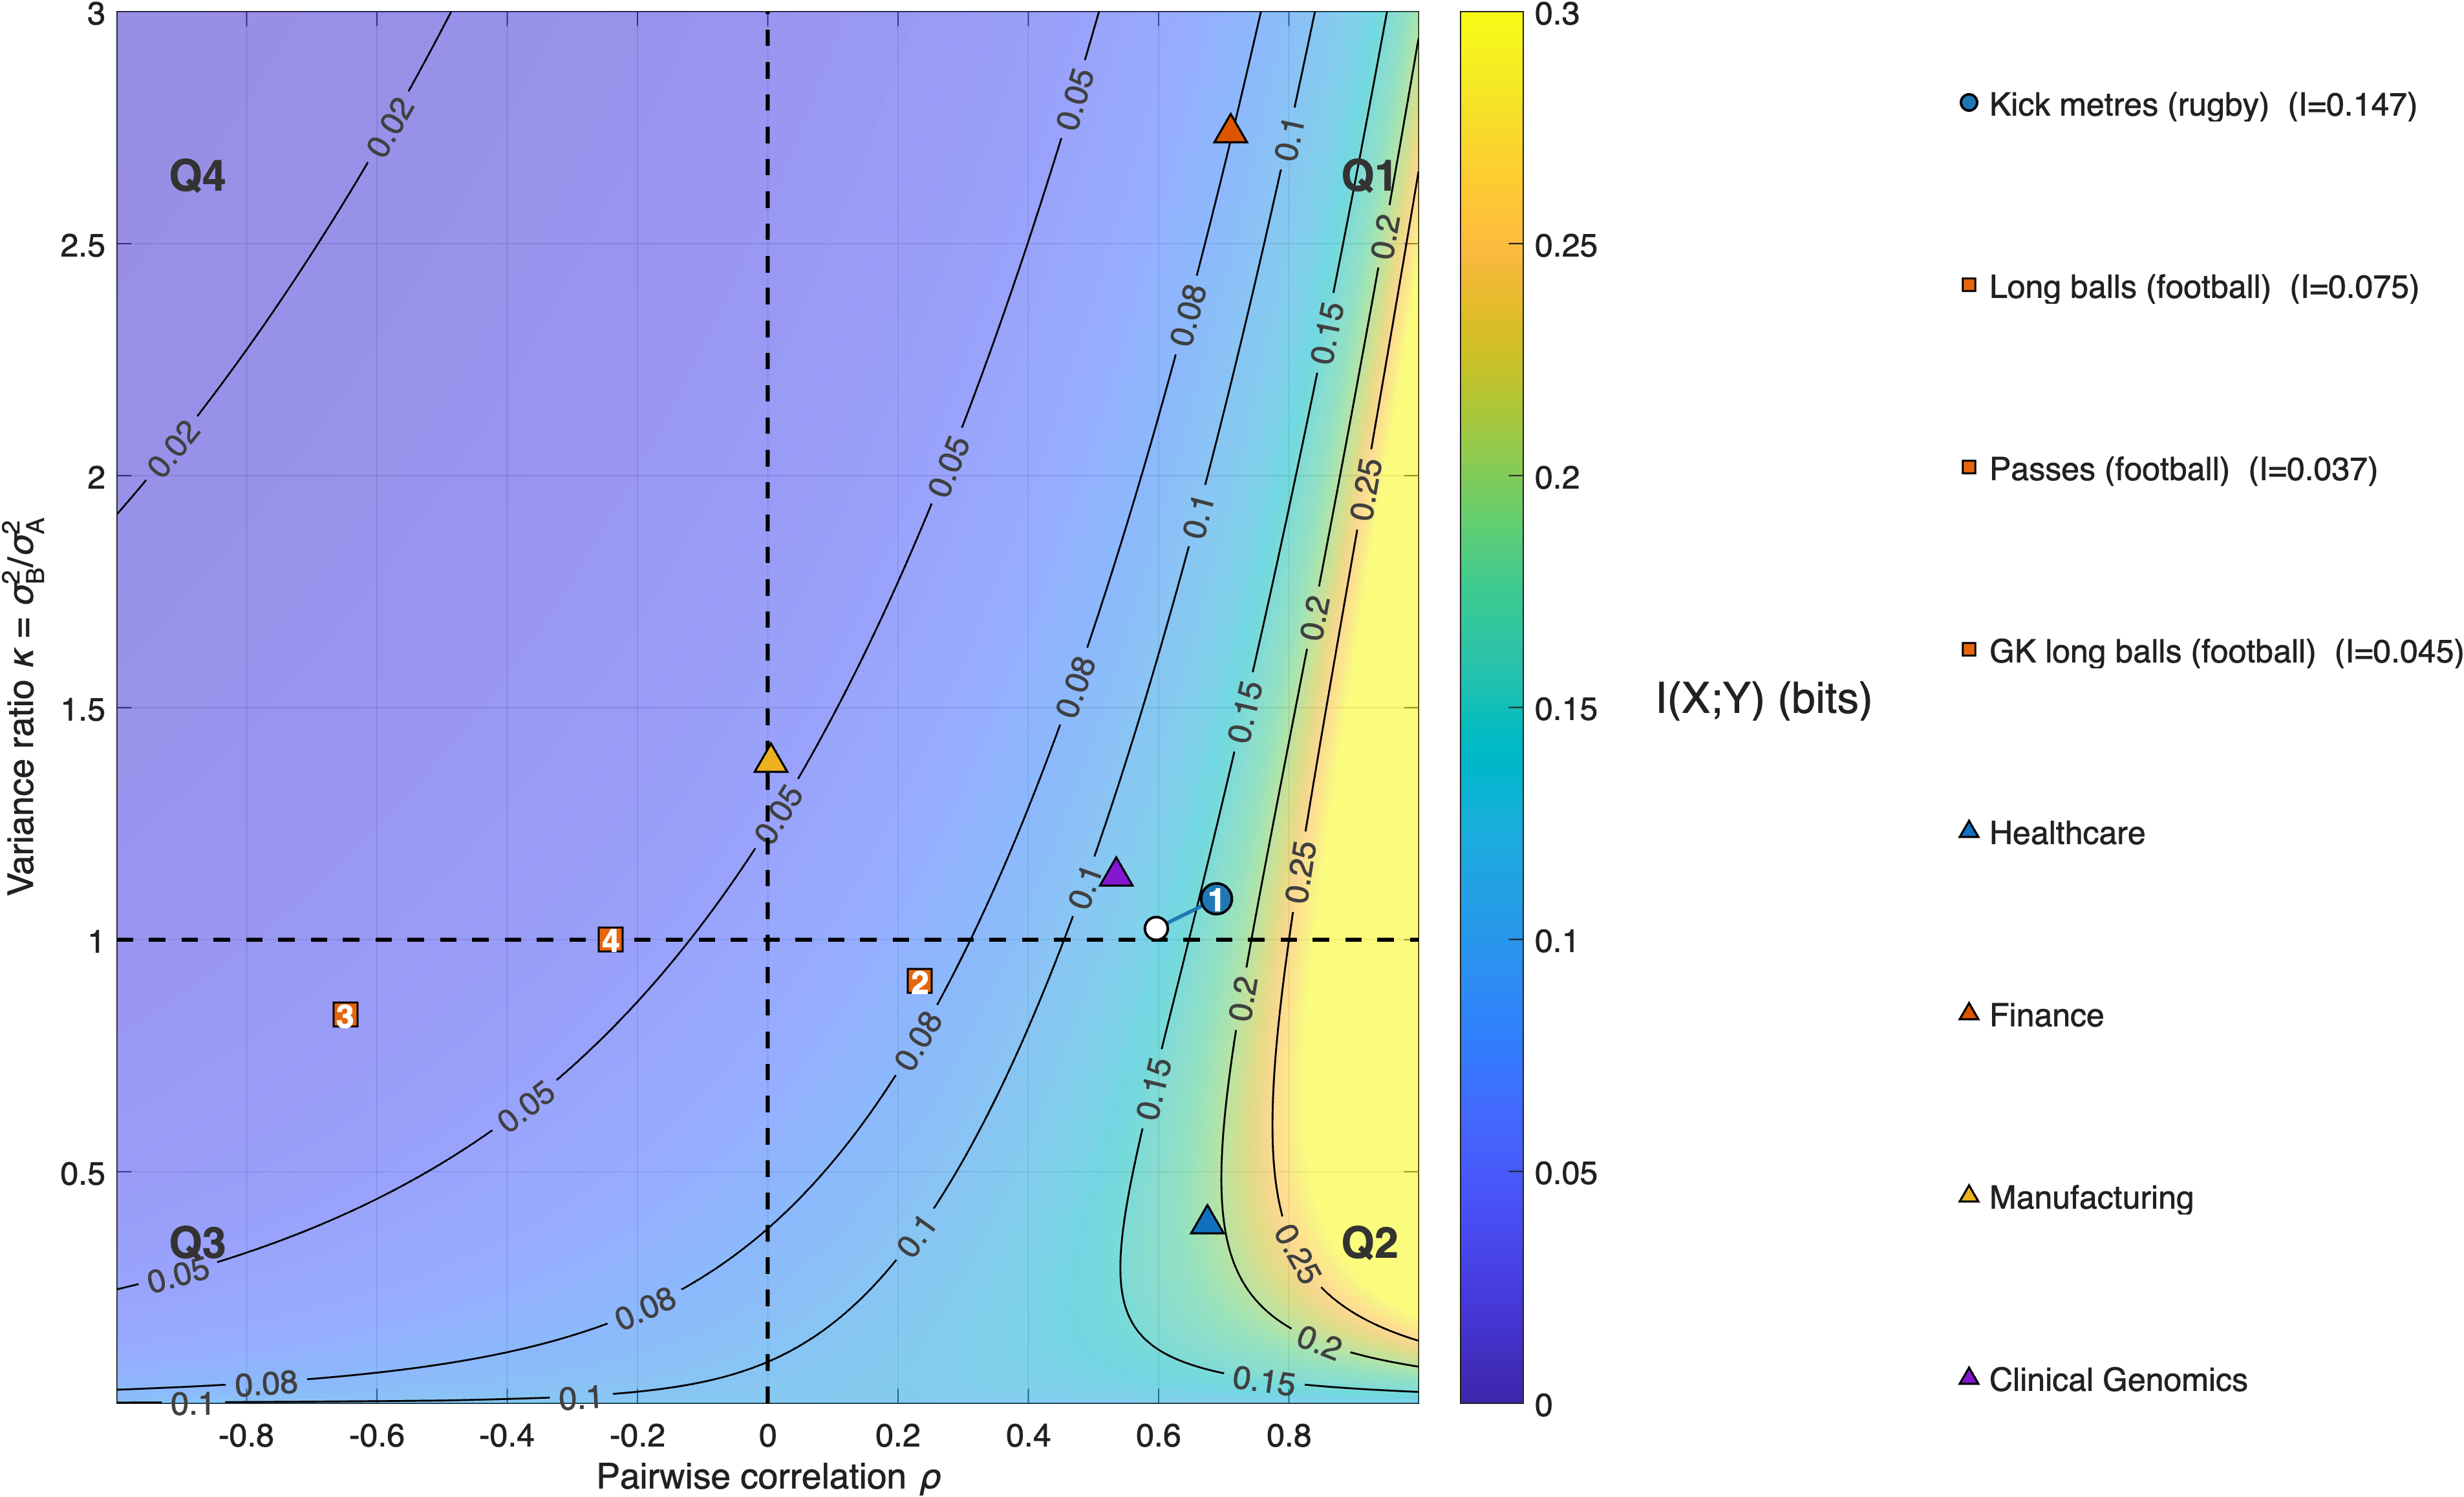
\includegraphics[width=0.95\linewidth]{figures/Figure_2.png}
  \caption{Information-theoretic surface $I(X;Y)$ as a function of $\rho$ and $\kappa$
    (\cref{eq:mi_closed}), computed with nominal signal strength $\delta/\sigma_{\mathrm{A}}=1$.
    Layout matches \cref{fig:pef_landscape}: the same four confirmatory exemplars
    (\cref{tab:exemplars}) are plotted at their estimated $(\kappa,\rho)$ positions on this
    $\delta/\sigma_{\mathrm{A}}=1$ surface, with season 23/24--24/25 drift segments, supporting-domain triangles,
    quadrant boundaries, and the admissibility boundary (dotted curve).
    Background shading uses a \emph{sequential} colour scale over $I(X;Y)\in[0,0.3]$~bits
    (low to high information); \cref{fig:pef_landscape} uses a \emph{diverging}
    $\log_{10}$ scale of $\eta$ centred on the efficiency boundary $\eta=1$.
    Sensitivity to $\delta/\sigma_{\mathrm{A}}\in\{0.5,1.0,2.0\}$ appears in
    Supplementary~\cref{fig:si_info_sensitivity}.}
  \label{fig:info_surface}
\end{figure}

\begin{figure}[p]
  \centering
  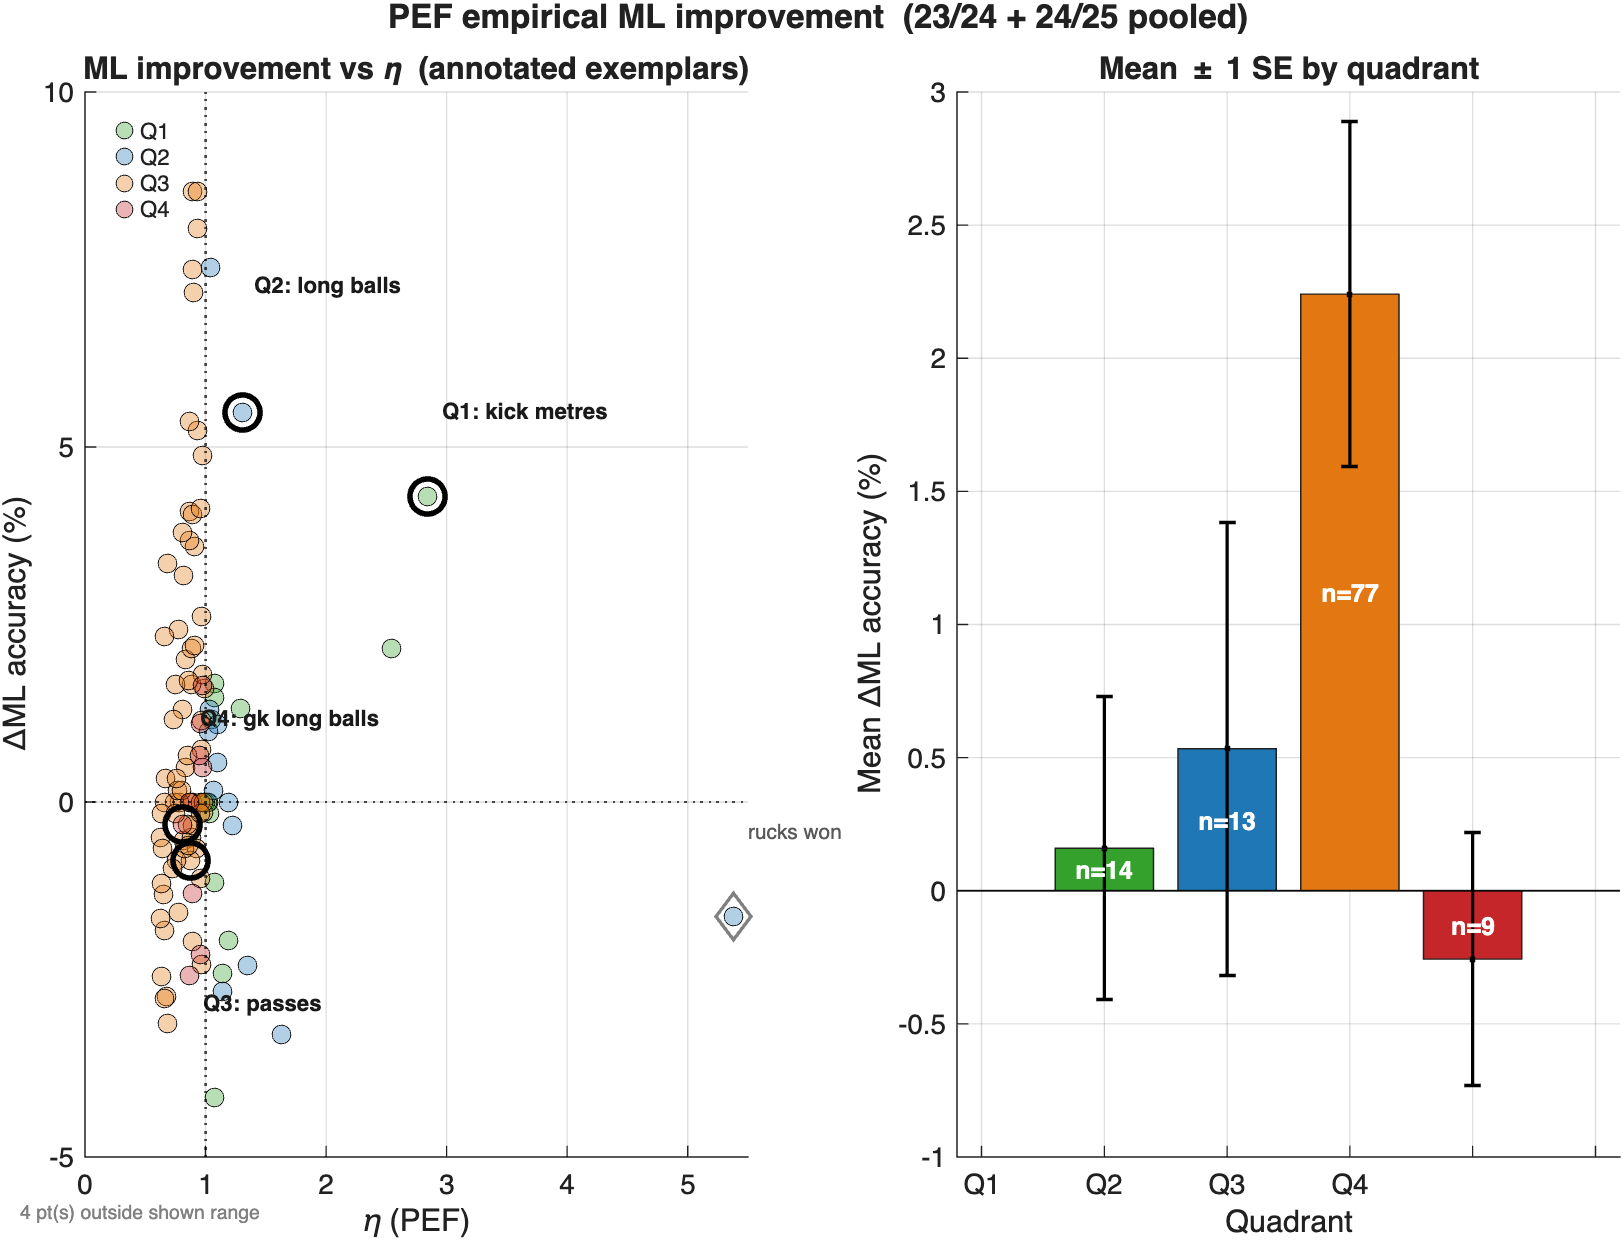
\includegraphics[width=0.72\linewidth]{figures/Figure_3.png}
  \caption{Confirmatory machine-learning check: $\Delta\mathrm{ML}$ versus $\hat\eta$ for four quadrant exemplars at comparable $\delta/\sigma_{\mathrm{A}}$ (\cref{tab:exemplars}).
    $\Delta\mathrm{ML}=100(\mathrm{acc}_{\mathrm{rel}}-\mathrm{acc}_{\mathrm{abs}})/\mathrm{acc}_{\mathrm{abs}}$ from team-blocked five-fold CV logistic regression (\cref{sec:ml_cv}).
    The zero line is the decision: above it, use the relative feature; below it, keep the absolute feature.
    Direction at matched signal: Q1 and Q2, $\eta>1$ with $\Delta\mathrm{ML}>0$; Q3, $\eta<1$ with $\Delta\mathrm{ML}<0$; Q4, $\eta<1$ with near-zero $\Delta\mathrm{ML}$.
    Rucks won (diamond) is a high-$\eta$ foil with negligible $\delta/\sigma_{\mathrm{A}}$: pairing efficiency without signal still yields $\Delta\mathrm{ML}<0$.
    The $x$-axis is broken between $3.4$ and $5.05$ to keep the foil on scale.
    Colours match \cref{fig:pef_landscape,fig:info_surface}.
    The full inventory, including cases with $\eta<1$ and $\Delta\mathrm{ML}>0$, is in Supplementary~\cref{fig:si_kpi_labelled,fig:si_ipred_vs_dml}.}
  \label{fig:pef_ml}
\end{figure}

